% --------------------------------------------------------------------------
% Template for DCASE 2016 paper; to be used with:
%          dcase2016.sty  - DCASE 2016 LaTeX style file, and
%          IEEEbib.bst - IEEE bibliography style file.
% Adapted from spconf.sty and waspaa15.sty
% --------------------------------------------------------------------------

\documentclass{article}
\usepackage{dcase2016,amsmath,graphicx,url,times}
%\usepackage{dcase2016,amssymb,amsmath,graphicx,times,url}

% Example definitions.
% --------------------
\def\defeqn{\stackrel{\triangle}{=}}
\newcommand{\symvec}[1]{{\mbox{\boldmath $#1$}}}
\newcommand{\symmat}[1]{{\mbox{\boldmath $#1$}}}

% Title.
% --------------------
\title{Estimating traffic noise level using acoustic monitoring : a preliminary study}

% Single addresses (uncomment and modify for single-address case).
% --------------------
%\name{Author(s) Name(s)\thanks{Thanks to XYZ agency for funding.}}
%\address{Author Affiliation(s)}
%
% For example:
% ------------
%\address{School\\
%       Department\\
%       Address}

% Two addresses
% --------------------
\twoauthors
  {Jean-R\'emy Gloaguen}
    {Ifsttar - LAE\\
	Route de Bouaye - CS4\\
     Bouguenais, 44344 , FR \\
     jean-remy.gloaguen@ifsttar.fr}
  {Arnaud Can}
    {Ifsttar - LAE\\
	Route de Bouaye - CS4\\
     Bouguenais, 44344 , FR \\
     arnaud.can@ifsttar.fr}
%  {Mathieu Lagrange}
%    {Irccyn\\
%	1 rue de la Noë\\
%     Nantes, 44321 , FR \\
%     mathieu.lagrange@irccyn.ec-nantes.fr}
%  {Jean-François Petiot}
%    {Irccyn\\
%	1 rue de la Noë\\
%     Nantes, 44321 , FR \\
%     jean-françois.petiot@irccyn.ec-nantes.fr}

\begin{document}

\ninept
\maketitle

\begin{sloppy}

\begin{abstract}
%  In order to help authors prepare their manuscripts for 
%  submission to DCASE 2016 and generate IEEE Xplore-compatible 
%  PDFs, we compile a list of guidelines and put together two
%  templates for users of both \LaTeX\ and Microsoft Word, which
%  can be downloaded from the workshop website at \cite{dcase2016web}.
%  These guidelines and templates are modified from those for past
%  ICASSP and WASPAA workshops, so an experienced author who 
%  has published something in these conferences/workshops will 
%  find it easy to follow the guidelines and use the templates.
\end{abstract}

\begin{keywords}
One, two, three, four, five
\end{keywords}

\section{Introduction}
\label{sec:intro}

Gêne 
Contexte normatif
motivation (rapide)
structure du papier


\section{Motivations}
\label{sec:format}

Norme europe
modèle de propagation
Réseaux de capteurs pas cher
besoin de calibration des modèles de propa
utilisation brut des données

\section{Method}
To seek this problem, we use the nonnegative matrix factorization \cite{lee1999} (NMF). This dimension-reduction technique consists in 

\begin{equation}\label{eq:NMF}
\mathbf{V} \approx \mathbf{WH}
\end{equation}

where $\mathbf{V}$, $F \times N$, is the power spectrogram of an audio, $\mathbf{W}$, $F \times K$, is the basis matrix and $\mathbf{H}$, $K \times N$, is the feature matrix. This approximation method is used for multiple applications as learning parts of images or text \cite{lee1999}, for polyphonic music transcription \cite{smaragdis2003}...
The approximation \ref{eq:NMF} is determined by a minimization problem

\begin{equation}\label{eq:minCost}
\underset{\mathbf{W},\mathbf{H} \geq 0}{\text{min }} D(V\vert\vert WH).
\end{equation}

$D(V\vert\vert WH)$ is called function cost and can take different forms \cite{amari2010}. In this study, we keep the most popular expressions which belong to the class of Bregman divergences and to the sub-class of $\beta$-divergence, the euclidian distance ($\beta = 2$)

\begin{equation}\label{eq:distEUC}
D_{EUC}(V\vert\vert WH) = \|\| V- WH \|\|, 
\end{equation} 

the Kullback-Leibler divergence, ($\beta = 1$), 

\begin{equation}\label{eq:divKL}
D_{KL}(V\vert\vert WH) = \mathbf{V}\log\frac{\mathbf{V}}{\mathbf{WH}}-\mathbf{V}+\mathbf{WH},
\end{equation}

and the Itakura-Saïto divergence, ($\beta = 0$), 
 
\begin{equation}\label{eq:divIS}
D_{IS}(V\vert\vert WH) = frac{\mathbf{V}}{\mathbf{WH}} -\log\frac{\mathbf{V}}{\mathbf{WH}}-1.
\end{equation}

In the case of unsupervised NMF, (\ref{eq:minCost}) is resolved iteratively where $\mathbf{W}$ is update in first for $\mathbf{H}$ fixed and then $\mathbf{H}$ is update with the new $\mathbf{W}$ fixed. Here, we considered the supervised NMF where $\mathbf{W}$ is fixed and only $\mathbf{H}$ is updated.

Different algorithms were developped to proposed an update of $\mathbf{H}$ with the prove of convergence \cite{lee2001} \cite{amari2011}. The choosen method is the maximisation-minimisation algorithm proposed by F\'{e}votte and Idier \cite{fevotte2011}.

\begin{equation}
\mathbf{H} = \mathbf{H}\left(\frac{\mathbf{W}^T\left[\mathbf{WH}^{\beta-2}.\mathbf{V} \right]}{W^T \left[ \mathbf{WH} \right]^{\beta-1}}\right)^{\gamma(\beta)}
\end{equation}

where $\gamma(\beta) = 1$ for $\beta \in [1 2]$ and $\gamma(\beta) = \dfrac{1}{2}$ for $\beta = 0$. Currently, $H$ is updated for a number of iteration fixed at 100.

When the iteration is over, for each temporal frame, the traffic sound level is calculated with the element related to traffic $\mathbf{\tilde{V}}_{traffic} = \mathbf{WH}_{traffic}$,

\begin{equation}
L_{p,n} = 20\log\frac{\sum\mathbf{v_{n_{traffic}}}}{p_ref}
\end{equation}

with $\tilde{v}_n$, the $n$-th frame of matrix $V$ and $ p_{ref} = 2\times 10^{-5}$ Pa, the sound pressure reference. The equivalent trafic sound level, $L_{eq,tr}$ (\ref{eq:Leq}) is then determined by

\begin{equation}
L_{eq,tr} = \frac{1}{T} \sum 10\log (10^{L_{p,n}/10}
\end{equation}

where $T$ is the duration of $\mathbf{V}$.\\

The choice of using the NMF is justified by the consideration of overlap between the sound sources, the ease to implement this method and that it was never used for this kind of sound environnement.

\section{Experiment}

To tested the NMF, synthetized sounds mixtures are used and not real measurements. In these, the real traffic sound level, $L_{eq,tr}$, is not correctly known and can be overlap with other sound sources not related. The comparison between $L_{eq,tr}$ and the estimated $\tilde{L}_{eq,tr}$ would be incorrect. Furthermore, working on sound mixtures simulated will create a controled framework.
The mixtures are realized by \textit{simScene} created by Mathias Rossignol and Gregoire Lafay \cite{simScene} synthetized sound mixtures from a sound data base. This tool can control multiple parameters as the event/background ratio, the sample duration, the time between samples \dots Each of these parameters are coupled with a standart deviation to bring some variability between the scenes produced. In the ouput, an audio file of the mix and for each sound class too is created. This allows to know the specific contribution of each class, in our case it is the traffic. The sound data base we use is composed of sound samples provided by the author completed by others sounds found online (\textit{freesound.org}). The scenes are realized with the first half of the data base, the second half will be used in the basis matrix $\mathbf{W}$.\\

For this preliminary study, 20 scenes were created with a duration of 15 s. Each is composed of 3 classes of sound we can typically ear in town : \textit{car}, \textit{bird} and \textit{horn}. The aim of this preliminary study is to see the influence of some parameters of the NMF on the quality of the traffic noise level estimation (the divergence calculation, the number of iteration).\\
% and the number of class in $\mathbf{W}$).\\

The aim is to execute an NMF on each scene to compare 
the equivalent sound level of traffic, $L_{eq,tr}$ with the estimation given by the NMF $\tilde{L}_{eq,tr}$.
Then, to evaluate the performance of the method, the RMSE is considered

\begin{equation}
RSME = \sqrt{\sum_{i = 1}^N((L^i_{eq,tr}-\tilde{L}^i_{eq,tr})^2}
\end{equation}

Figure \ref{fig:spectrogram} resumes the spectrograms obtained by simScene (on left) and by the NMF (on right) for one scene with euclidian distance (\ref{eq:distEUC}) after 100 updates of $\mathbf{H}$. We can observe the bird on the frequence range $\left[3000-6000\right]$ Hz, the horn is characterized by its harmonic content whereas the car is principally composed of bass frequencies with a slower temporal evolution.

\begin{figure}[btp]
\centering
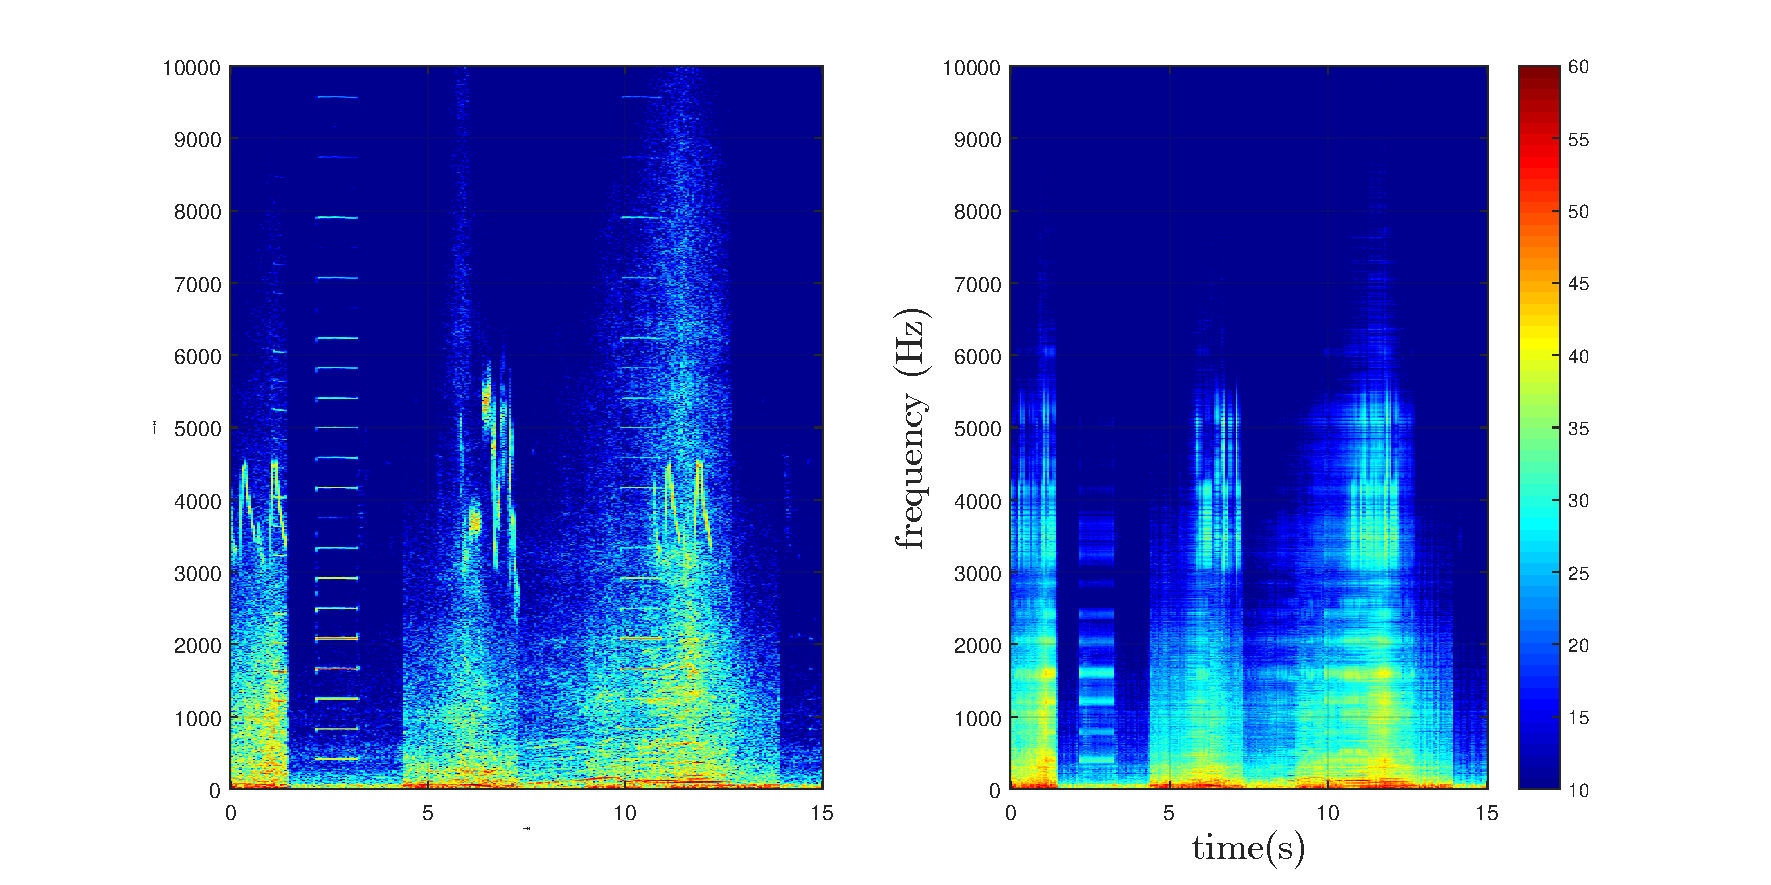
\includegraphics[scale=0.25]{./images/bvak_Sc2_V_spectre_Euc.pdf}
\caption{Spectrograms of a sound mixture composed with 3 sound classes (car, horn, bird). On the left, the audio gives by simScene, on the right, one obtained with NMF}
\label{fig:spectrogram}
\end{figure}

From each sound mixture, comparison between $L_{p,t}$ and $\tilde{L}_{p,t}$ for Euclidian distance, Kullback-Leibler and Itakura-Saïto divergences can be made (figure~\ref{fig:Lp}

\begin{figure}[btp]
\centering
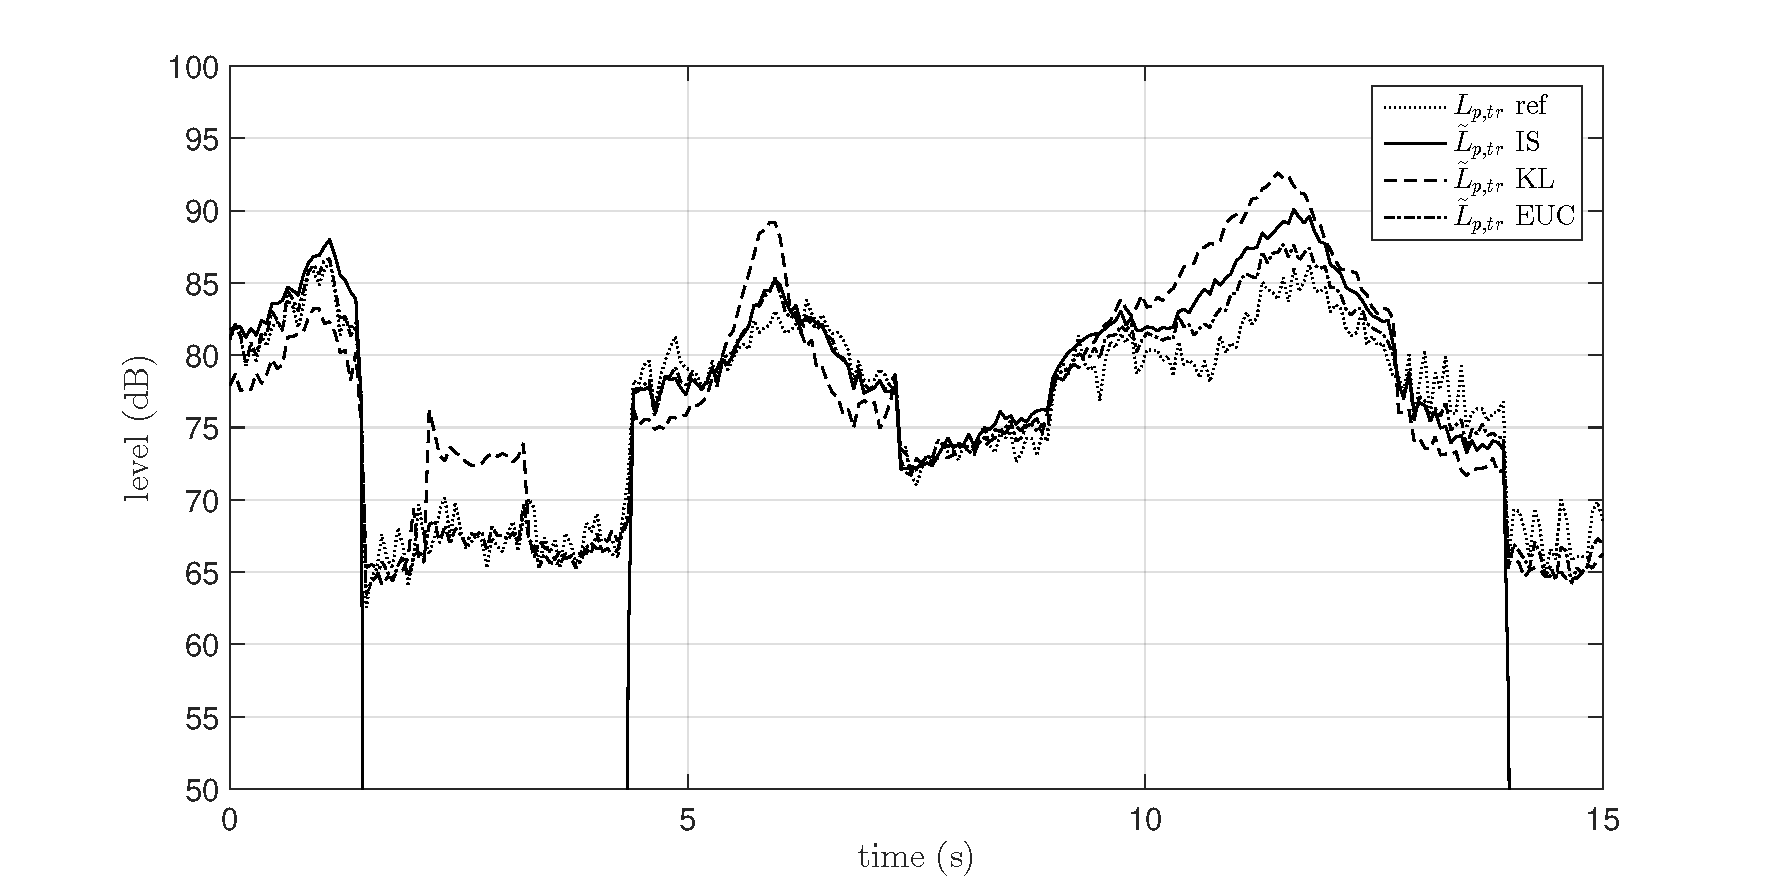
\includegraphics[scale=0.25]{images/Lp_bvak_Sc2_It98_nbCl3.pdf}
\caption{Sound pressure level estimated and real of one scene for the distance and the two divergences}
\label{fig:Lp}
\end{figure}

The RMSE is calculated in terms of iterations for the three divergences. The error between $L_{eq,tr}$ and the equivalent sound pressure of the global mixture is added. This resumes the error caused if the source separation is not realized and all sound sources are taken account without distinction.

\begin{figure}[btp]
\centering
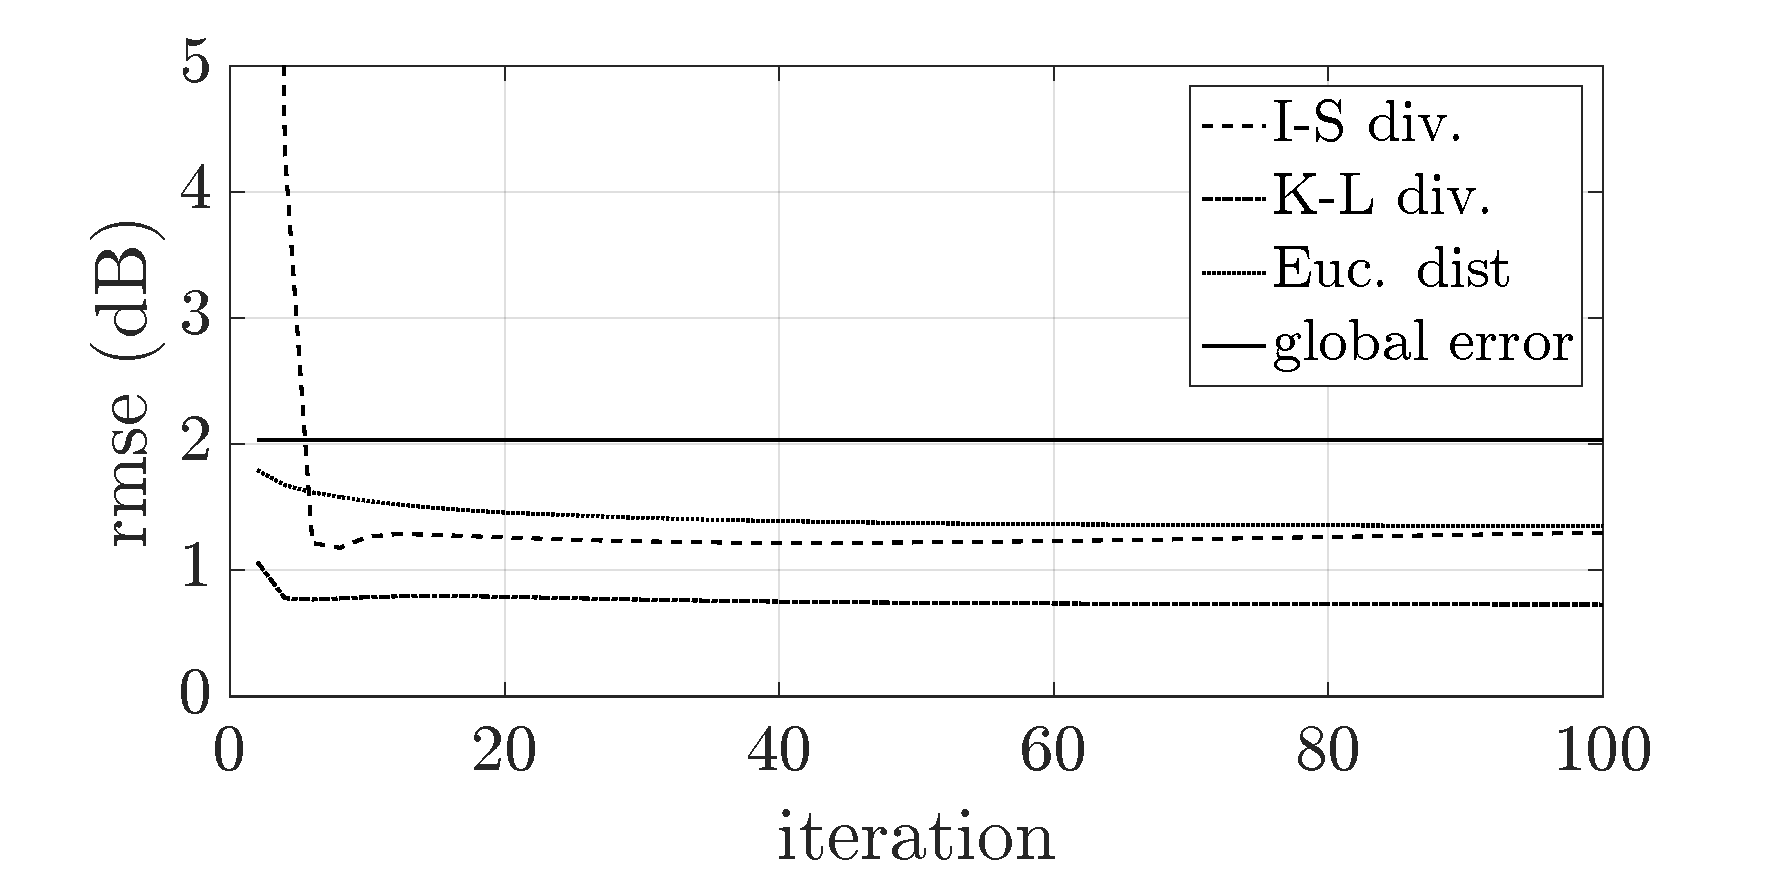
\includegraphics[scale=0.25]{images/comparaison_RMSE_nbCl3.pdf}
\caption{RMSE evolution}
\label{fig:rmse}
\end{figure}

The application of the NMF to calculate the traffic noise level, in all cases, produce a better estimation than taking the sound mixture with all the sound source. The Kullback-Leibler divergence proposed the most interesting results with the lowest and the most stable RMSE.


\section{Conclusion}
In this article, we proposed the use of the supervised NMF to estimate the traffic noise level in city to improve the noise mapping with measurements. This method consist in the approximation of the spectrogram of the measure by the product between two matrices : $W$, composed of spectra of differents sound sources found in an urban area, and $H$,  bringing the temporal variation of each spectrum. By taking account of the \textit{traffic} element, an traffic noise level estimation is obtained. This method is tested on sound mixtures created by the simScene software which gave us the traffic contribution separately from the other sounds. By comparing the equivalent sound level between the traffic element of simScene and the estimation given by the NMF for three cost functions, the quality of this method is tested. The first results show that this method gives a better estimation of the sound level than if the source separation is not done proving its interest. Furthermore, it shows that the Kullback-Leibler divergence propose the lowest error and seems the fittest cost function to use for our futur tests.


%All manuscripts must be submitted electronically as PDF files. 
%All manuscripts must be formatted for white US letter paper 
%(8.5 $\times$ 11 inches). Please do {\bf not} use A4-size papers. 
%All printed material, including text, illustrations, and charts, 
%must be kept within a print area of 7.0 inches (178 mm) wide 
%by 8.9 inches (226 mm) high. Do not write or print anything outside 
%the print area. The top margin must be 1 inch (25 mm), except for 
%the title page, and the left margin must be 0.75 inch (19 mm).  
%All {\it text} must be in a two-column format. Columns are to be 
%3.29 inches (83.5 mm) wide, with a 0.31 inch (8 mm) space between 
%them. Text must be fully justified. 
%
%
%\section{NUMBER OF PAGES}
%\label{sec:pagelimit}
%
%You are allowed a total of up to 4+1 pages for your DCASE 2016 Challenge 
%and Workshop submissions, with up to 4 pages for technical content including 
%figures and possible references, with the optional 5th page containing only
%references. 
%
%\section{PAGE TITLE SECTION}
%\label{sec:pagestyle}
%
%The paper title (on the first page) should begin 0.98 inches 
%(25 mm) from the top edge of the page, centered, completely 
%capitalized, and in Times 14-point, boldface type.  
%The authors' name(s) and affiliation(s) appear below the title
%in capital and lower case letters.  Papers with multiple authors 
%and affiliations may require two or more lines for this information.
%
%\section{TYPE-STYLE AND FONTS}
%\label{sec:typestyle}
%
%We strongly encourage you to use Times-Roman 
%font. In addition, this will give the proceedings a more uniform 
%look. Use a font that is no smaller than nine point type 
%throughout the paper, including figure captions.
%
%In nine point type font, capital letters are 2 mm high.  
%{\bf If you use the smallest point size, there should be 
%no more than 3.2 lines/cm (8 lines/inch) vertically.}  
%This is a minimum spacing; 2.75 lines/cm (7 lines/inch) 
%will make the paper much more readable. Larger type sizes 
%require correspondingly larger vertical spacing. Please do 
%not double-space your paper. True-Type 1 fonts are preferred.
%
%The first paragraph in each section should not be indented, 
%but all the following paragraphs within the section should 
%be indented as these paragraphs demonstrate.
%
%\section{MAJOR HEADINGS}
%\label{sec:majhead}
%
%Major headings, for example, ``1. Introduction'', should 
%appear in all capital letters, bold face if possible, 
%centered in the column, with one blank line before, 
%and one blank line after. Use a period (``.'') after 
%the heading number, not a colon.
%
%\subsection{Subheadings}
%\label{ssec:subhead}
%
%Subheadings should appear in lower case (initial word 
%capitalized) in boldface. They should start at the left 
%margin on a separate line. 
% 
%\subsubsection{Sub-subheadings}
%\label{sssec:subsubhead}
%
%Sub-subheadings, as in this paragraph, are discouraged. 
%However, if you must use them, they should appear in 
%lower case (initial word capitalized) and start at the 
%left margin on a separate line, with paragraph
%text beginning on the following line. They should be 
%in italics. 
% 
%
%\section{Page Numbering, Header, and Footer}
%\label{sec:page}
%
%Please do {\bf not} paginate your paper. 
%In addition, please do {\bf not} change and remove
%the header and footer.
%
%\section{ILLUSTRATIONS, GRAPHS, AND PHOTOGRAPHS}
%\label{sec:illust}
%
%Illustrations must appear within the designated margins.  
%They may span the two columns. If possible, position 
%illustrations at the top of columns, rather than in 
%the middle or at the bottom. Caption and number every 
%illustration. All halftone illustrations must be clear 
%black and white prints. Colors may be used, but they 
%should be selected so as to be readable when printed 
%on a black-only printer.
%
%Since there are many ways, often incompatible, of 
%including images (e.g., with experimental results) 
%in a \LaTeX\ document, an example of how to do
%this is presented in Fig.~\ref{fig:results}.
%
%% Below is an example of how to insert images. 
%% -------------------------------------------------------------------------
%%\begin{figure}[t]
%%  \centering
%%  \centerline{\includegraphics[width=\columnwidth]{fig1a}}
%%  \caption{Example of a figure with experimental results.}
%%  \label{fig:results}
%%\end{figure}
%
%\section{Equations}
%\label{sec:equations}
%
%Equations should be placed on separate lines and consecutively
%numbered with equation numbers in parentheses flush with the 
%right margin, as illustrated in (\ref{eqn:wave_equation}) 
%that gives the homogeneous acoustic wave equation in
%Cartesian coordinates \cite{eWilliams1999},
%\begin{equation}
%  \label{eqn:wave_equation}
%    \Delta^2p(x,y,z,t)-
%    \displaystyle\frac{1}{c^2}\frac{\partial^2p(x,y,z,t)}{\partial t^2}=0,
%\end{equation}
%where $p(x,y,z,t)$ is an infinitesimal variation of acoustic 
%pressure from its equilibrium value at position $(x,y,z)$ and 
%time $t$, and where $c$ denotes the speed of sound.
%
%Symbols in your equation should be defined before the equation 
%appears or immediately following.  Use (1), not Eq. (1) or 
%equation (1), except at the beginning of a sentence:  
%``Equation (1) is ...''
%
%
%
%\section{FOOTNOTES}
%\label{sec:foot}
%
%Use footnotes sparingly and place them at 
%the bottom of the column on the page on which they are 
%referenced. Use Times 9-point type, single-spaced. To 
%help your readers, avoid using footnotes altogether and
%include necessary peripheral observations in the text 
%(within parentheses, if you prefer, as in this sentence).
%
%\section{REFERENCES}
%\label{sec:ref}
%
%List and number all bibliographical references at the end 
%of the paper. The references should be numbered in order 
%of appearance in the document. When referring to them in 
%the text, type the corresponding reference number in 
%square brackets as shown at the end of this sentence 
%\cite{cJones2003}, \cite{aSmith2000}. For \LaTeX\ users, 
%the use of the Bib\TeX\ style file IEEEtran.bst is 
%recommended, which is included in the \LaTeX\ paper 
%kit available from the DCASE 2016 website \cite{dcase2016web}.
%
%\section{ACKNOWLEDGMENT}
%\label{sec:ack}
%
%The preferred spelling of the word acknowledgment in 
%America is without an ``e'' after the ``g.'' Try to avoid 
%the stilted expression, ``One of us (R. B. G.) thanks ...''
%Instead, try ``R.B.G.\ thanks ...''  Put sponsor 
%acknowledgments in the unnumbered footnote on the first page.

% -------------------------------------------------------------------------
% Either list references using the bibliography style file IEEEtran.bst
\bibliographystyle{IEEEtran}
\bibliography{refs}
%
% or list them by yourself
% \begin{thebibliography}{9}
% 
% \bibitem{dcase2016web}
%   \url{http://www.cs.tut.fi/sgn/arg/dcase2016/}.
%
% \bibitem{IEEEPDFSpec}
%   {PDF} specification for {IEEE} {X}plore$^{\textregistered}$,
%   \url{http://www.ieee.org/portal/cms_docs/pubs/confstandards/pdfs/IEEE-PDF-SpecV401.pdf}.
%
% \bibitem{PDFOpenSourceTools}
%   Creating high resolution {PDF} files for book production with 
%   open source tools, 
%   \url{http://www.grassbook.org/neteler/highres_pdf.html}.
%
% \bibitem{eWilliams1999}
% E. Williams, \emph{Fourier Acoustics: Sound Radiation and Nearfield Acoustic
%   Holography}. London, UK: Academic Press, 1999.
% 
% \bibitem{ieeecopyright}
%   \url{http://www.ieee.org/web/publications/rights/copyrightmain.html}.
%
% \bibitem{cJones2003}
% C. Jones, A. Smith, and E. Roberts, ``A sample paper in conference
%   proceedings,'' in \emph{Proc. IEEE ICASSP}, vol. II, 2003, pp. 803--806.
% 
% \bibitem{aSmith2000}
% A. Smith, C. Jones, and E. Roberts, ``A sample paper in journals,'' 
%   \emph{IEEE Trans. Signal Process.}, vol. 62, pp. 291--294, Jan. 2000.
% 
% \end{thebibliography}


\end{sloppy}
\end{document}
